\documentclass[twocolumn,a4j]{jsarticle}
\setlength{\topmargin}{-20.4cm}
\setlength{\oddsidemargin}{-10.4mm}
\setlength{\evensidemargin}{-10.4mm}
\setlength{\textwidth}{18cm}
\setlength{\textheight}{26cm}

\usepackage[top=15truemm,bottom=20truemm,left=20truemm,right=20truemm]{geometry}
\usepackage[latin1]{inputenc}
\usepackage{amsmath}
\usepackage{amsfonts}
\usepackage{amssymb}
\usepackage[dvipdfmx]{graphicx}
\usepackage[hang,small,bf]{caption}
\usepackage[subrefformat=parens]{subcaption}
\usepackage[dvipdfmx]{color}
\usepackage{listings}
\usepackage{listings,jvlisting}
\usepackage{geometry}
\usepackage{framed}
\usepackage{color}
\usepackage[dvipdfmx]{hyperref}
\usepackage{ascmac}
\usepackage{enumerate}
\usepackage{tabularx}
\usepackage{cancel}
\usepackage{scalefnt}
\usepackage{overcite}
\usepackage{otf}
\usepackage{multicol}
\usepackage[geometry]{ifsym}

\renewcommand{\figurename}{Fig.}
\renewcommand{\tablename}{Table }

\hypersetup{%
    hidelinks %リンクの色消し
}

\lstset{
basicstyle={\ttfamily},
identifierstyle={\small},
commentstyle={\smallitshape},
keywordstyle={\small\bfseries},
ndkeywordstyle={\small},
stringstyle={\small\ttfamily},
frame={tb},
breaklines=true,
columns=[l]{fullflexible},
xrightmargin=0zw,
xleftmargin=3zw,
numberstyle={\scriptsize},
stepnumber=1,
numbersep=1zw,
lineskip=-0.5ex
}

% キャプション後ろのダブルコロンを消す
\makeatletter
\long\def\@makecaption#1#2{%
  \vskip\abovecaptionskip
  \iftdir\sbox\@tempboxa{#1\hskip1zw#2}%
    \else\sbox\@tempboxa{#1 #2}%
  \fi
  \ifdim \wd\@tempboxa >\hsize
    \iftdir #1\hskip1zw#2\relax\par
      \else #1 #2\relax\par\fi
  \else
    \global \@minipagefalse
    \hbox to\hsize{\hfil\box\@tempboxa\hfil}%
  \fi
  \vskip\belowcaptionskip}
\makeatother


\makeatletter
\def\@maketitle
{
\begin{center}
{\LARGE \@title \par}
\end{center}
\begin{flushright}
{\large \@date}\\
{\large 京都工芸繊維大学 大学院 機械設計学専攻 計測システム工学研究室}\\
{\large M2 \@author}
\end{flushright}
\par\vskip 1.5em
}
\makeatother

\author{来代 勝胤 / KITADAI Masatsugu}
\title{令和5年度 9月度 共同研究報告書}
\date{2023/09/29}

\begin{document}
\columnseprule=0.1mm
\maketitle

\section*{報告内容}
\begin{enumerate}[1.]
	\item ISTP-33 について
	\item 解析手順の再構成
	\item 10月の予定
\end{enumerate}

\section*{進捗報告}
今月は,9/24 - /27 まで ISTP-33 に参加し
研究発表を行った.
また,先月に引き続き,二次流れ解析プログラムの性能向上を目的に
アルゴリズムの見直しや処理の検討を行っている.

\section{ISTP-33 について}
\begin{table}[hbtp]
	\label{table:data_type}
	\begin{tabular*}{8cm}{ c | c }
		\hline
		\textgt{題目} & \begin{tabular}{c} Performance Evaluation \\ of PIV Measurement of Secondary Flow \\ using Multi-Color LLS \end{tabular}        \\ \hline
		\textgt{内容} & \begin{tabular}{c} 数値シミュレーションを用いた\\計測手法の精度評価の結果について \end{tabular}        \\ \hline
		\textgt{日時} & 2023/9/24 - 9/27                 \\ \hline
		\textgt{会場} & 熊本県 熊本市中央区 熊本城ホール\\ \hline
	\end{tabular*}
\end{table}

\section{解析手順の再構成}
これまで検討を行ってきた解析の一連の流れとアルゴリズムについて,
性能向上と解析手順の明確化のため見直しを行っている.

\begin{enumerate}[(1)]
	\item [] \textgt{[ 全体の流れ ]}
	\item 校正ブロックの校正点特定と補正関数の取得 (完了)
	\item 背景処理・粒子位置特定等の前処理 (完了)
	\item 粒子追跡 (検討中)
	\item ベクトルの再配置・誤ベクトル除去等の後処理 (検討中)
\end{enumerate}

\subsection{[3] 粒子追跡:同一粒子の判別}
レーザーシートを通過する粒子が複数枚の画像内に同一の粒子像が現れ,
流れ場の解析時に問題となる場合がある.
また,主流方向速度が局所的に変動する場合,粒子の追跡が困難となるため
おおよその粒子の持つ主流方向速度の情報を知る必要がある.

\newpage
そこで,今回は粒子像を画像の時刻経過に沿ってクラスタリングを行い,
その結果から粒子位置の特定や粒子の持つ速度情報の取得を試みた.

\begin{figure}[htbp]
	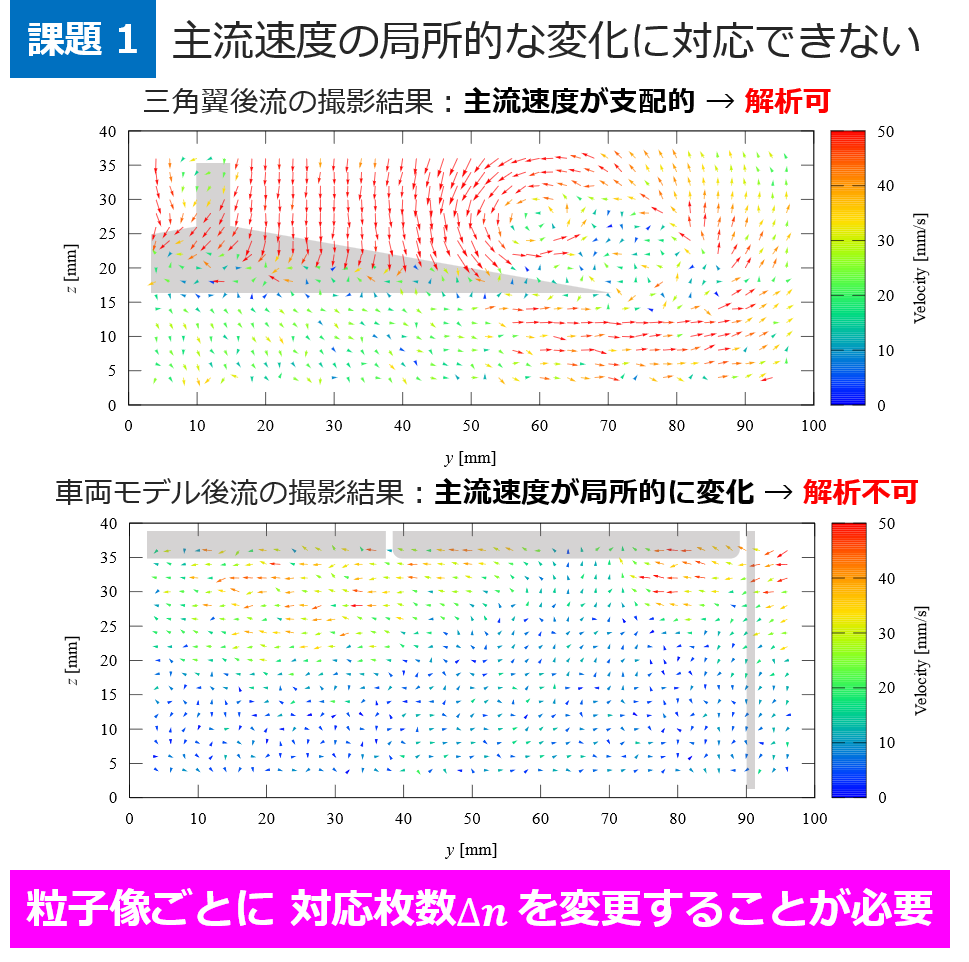
\includegraphics[keepaspectratio, width=80mm]{../images/challenge_1.png}
\end{figure}
\begin{figure}[htbp]
	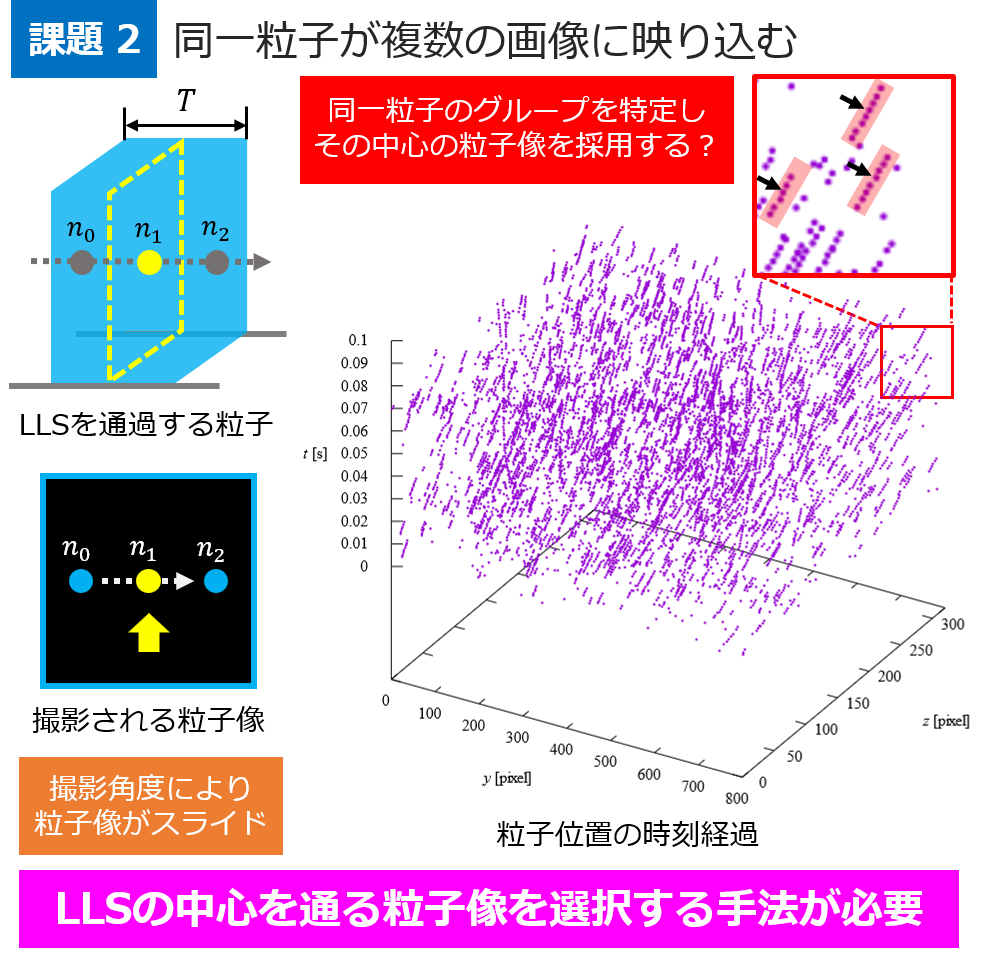
\includegraphics[keepaspectratio, width=80mm]{../images/challenge_2.png}
\end{figure}

\subsubsection*{粒子像のクラスタリング}
以下のFig.1は,各色の粒子像について,時刻ごとの粒子の移動を示している.
総じて時刻経過による移動量は非常に小さく,
傾向として時刻経過にしたがって右に移動することがわかる.
粒子の時刻経過の可視化結果から,同一粒子の判定には
最近法が有効であると考える.

\begin{figure}[htbp]
	\begin{tabular}{cc}
		\begin{minipage}[t]{0.45\hsize}
			\centering
			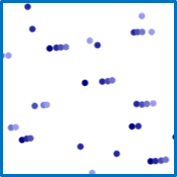
\includegraphics[keepaspectratio, width=32mm]{../images/time-line_blue.png}
			\subcaption{Blue}
		\end{minipage} &
		\begin{minipage}[t]{0.45\hsize}
			\centering
			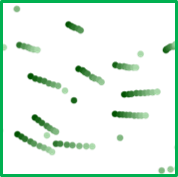
\includegraphics[keepaspectratio, width=32mm]{../images/time-line_green.png}
			\subcaption{Green}
		\end{minipage}
	\end{tabular}
	\caption{Particle Timeline}
\end{figure}

図2は,時刻経過画像に近法を用いてPTVを行い
クラスタリングを行った結果である.
このクラスタから,同一粒子を判定することができる.
\begin{figure}[htbp]
	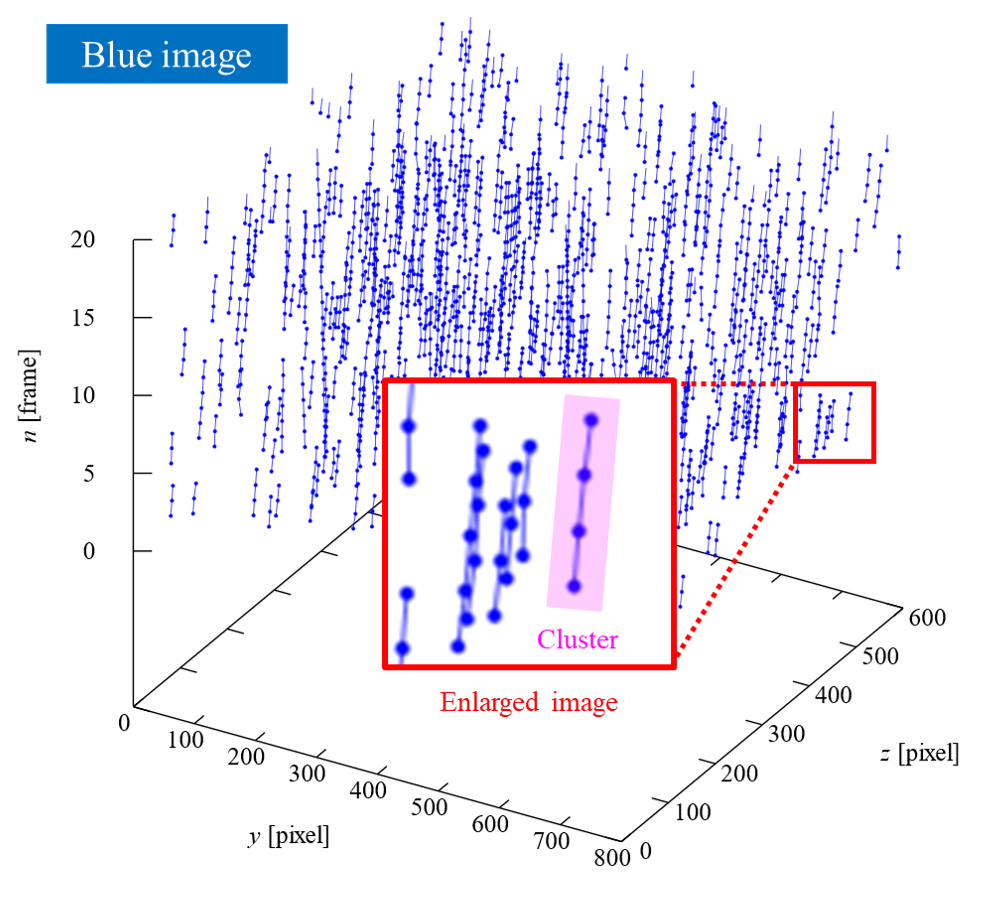
\includegraphics[keepaspectratio, width=85mm]{../images/cluster_for_b.png}
	\caption{Clustering for Blue Particle}
\end{figure}

\subsubsection*{粒子像の位置決定}
同一粒子の判定によって得られたクラスタから粒子位置の決定を行う.
ここで,$i$番目の粒子像は位置情報 $(y, z)$ と
撮影されたフレーム数 $n$ の3次元の情報を持ち,
それぞれの平均値を粒子情報$(y'_i, z'_i, n'_i)$として採用した.
\begin{eqnarray*}
	y'_i &=& \frac{1}{N_i} \sum_{j=1}^{N} y_{ij} \\
	z'_i &=& \frac{1}{N_i} \sum_{j=1}^{N} z_{ij} \\
	n'_i &=& \frac{1}{N_i} \sum_{j=1}^{N} n_{ij} \\
	i &:& \text{クラスタ番号}\\
	j &:& \text{フレーム番号}\\
	N_i &:& i \text{番目の粒子のフレーム総数}
\end{eqnarray*}

また,クラスタの粒子数 $N$ は
レーザーシート内に粒子が存在する時間を表していると考えられ,
粒子の主流方向速度 $u$ を以下の式から推定することができる.

\begin{eqnarray*}
	u_i &=& T \times \frac{f}{N_i}\\
	T &:& \text{レーザーシート厚み} \\
	f &:& \text{フレームレート}\\
\end{eqnarray*}
\subsubsection*{粒子追跡}
クラスタから得た粒子情報$(y', z', n', u)$から$u$を用いて,
後方のレーザーシートに到達するフレーム枚数差 $\Delta n$ を推定し,
最近値法を用いて粒子追跡を行う.
\begin{eqnarray*}
	\Delta n_i &=& \frac{\Delta x}{u_i} \\
	\Delta x &:& \text{レーザーシート間の距離}
\end{eqnarray*}

\begin{figure}[htbp]
	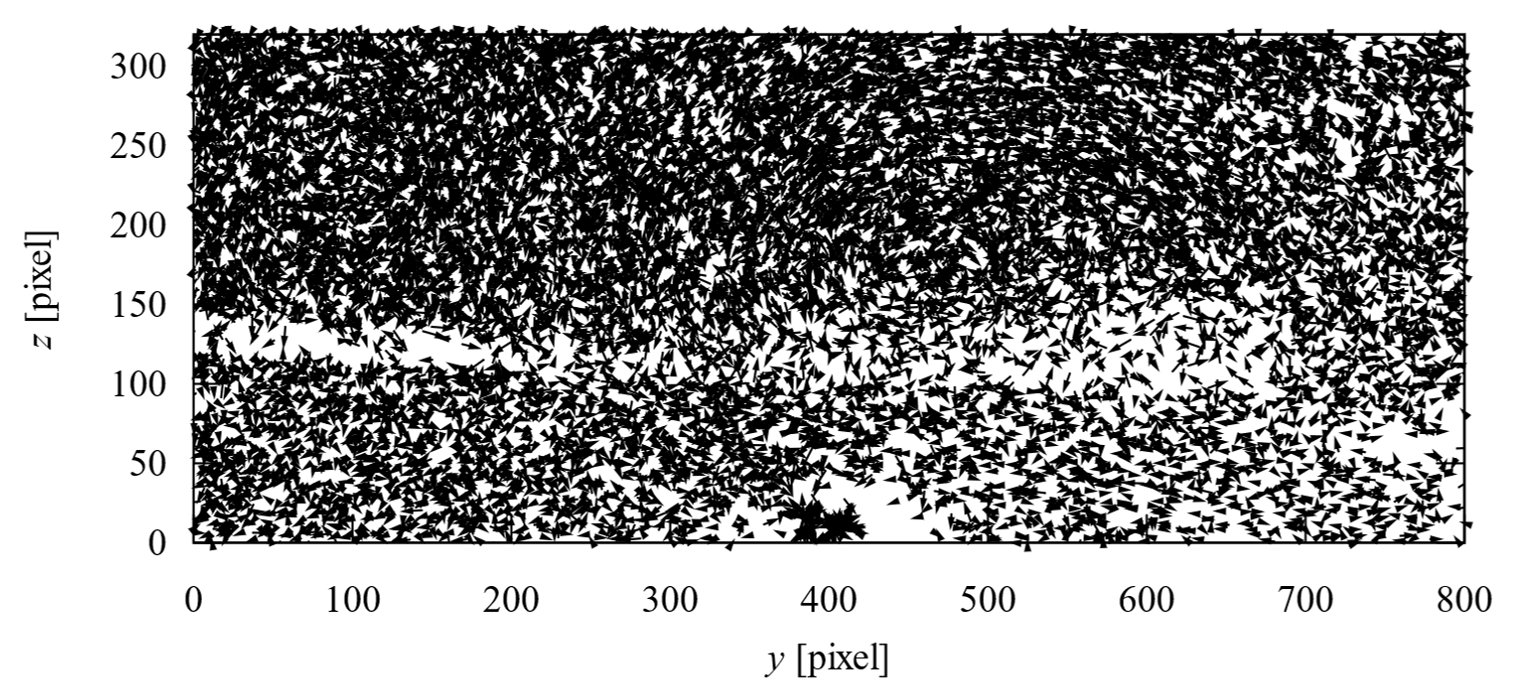
\includegraphics[keepaspectratio, width=85mm]{../images/cluster_matching.png}
	\caption{Particle tracking}
\end{figure}

\subsection{[4] ベクトルの再配置}
粒子マッチングの結果を用いて,ベクトルの再配置を行う.
解析されたすべての速度ベクトルを格子点からの距離に応じて
ガウス分布に従った重み付けを行い,速度ベクトルの推定を行う.
以下に再配置した結果を示す.

\begin{figure}[htbp]
	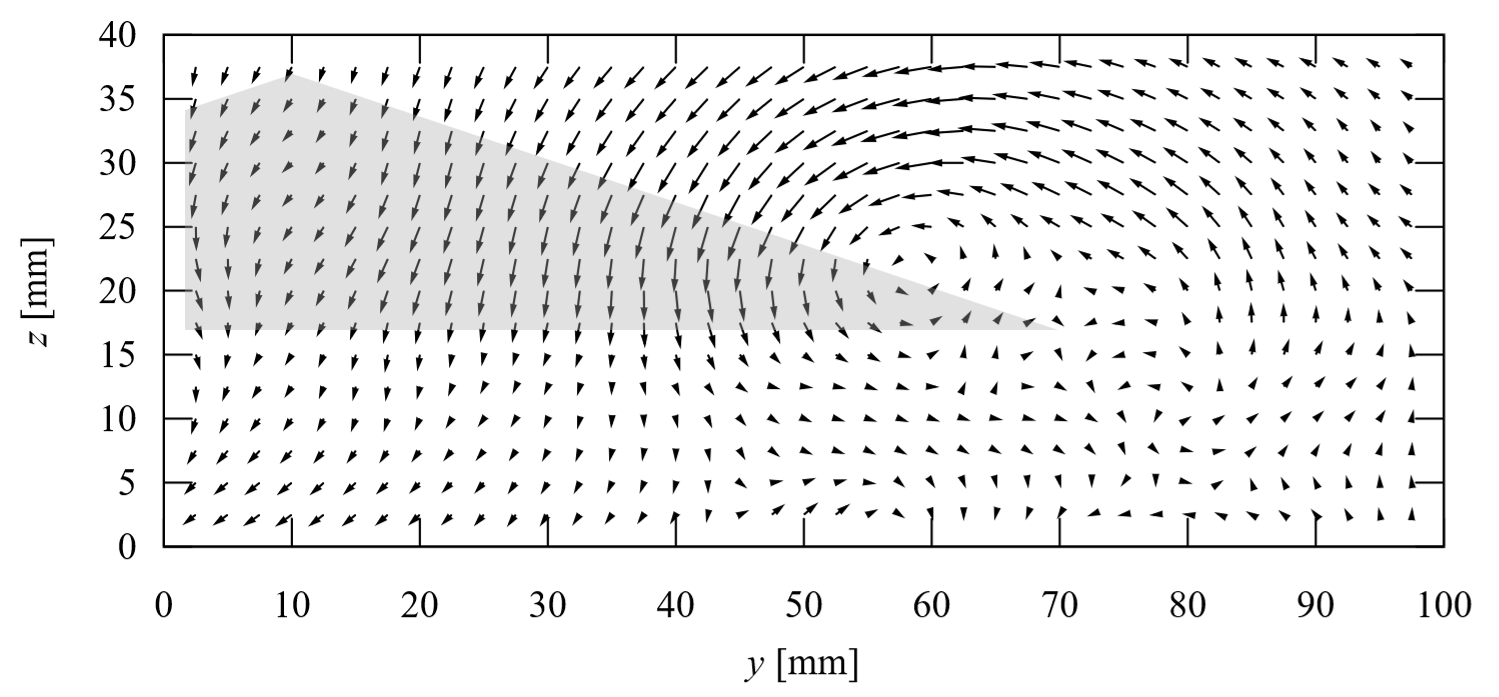
\includegraphics[keepaspectratio, width=85mm]{../images/time-averaged_velocity.png}
	\caption{Time-averaged velocity vector field}
\end{figure}

以前のアルゴリズムから推定した結果と同様に翼先端部に渦構造を確認することができる.
今後は,このアルゴリズムを用いて車両モデルの解析を行う.

\section{10月の予定}
\begin{itemize}
	\item 解析手順の再構成 (続き)
	\item 車両モデルの計測実験
\end{itemize}

\newpage
\begin{eqnarray*}
	n_{gi} &\geq& n_{bi} + \Delta n_i\\
	n_{bi} &:& 青色粒子像のフレーム数 [\#]\\
	n_{gi} &:& 緑色粒子像のフレーム数 [\#]
\end{eqnarray*}

\begin{table}[hbtp]
	\centering
	\begin{tabular}{l c}
		\hline
		Number of clustered blue particles  & 22102 \\ \hline
		Number of clustered green particles & 37956 \\ \hline
		Number of matched particle pairs    & 11668 \\ \hline
	\end{tabular}
\end{table}

\end{document}